% Created by tikzDevice version 0.12 on 2019-03-04 16:30:47
% !TEX encoding = UTF-8 Unicode
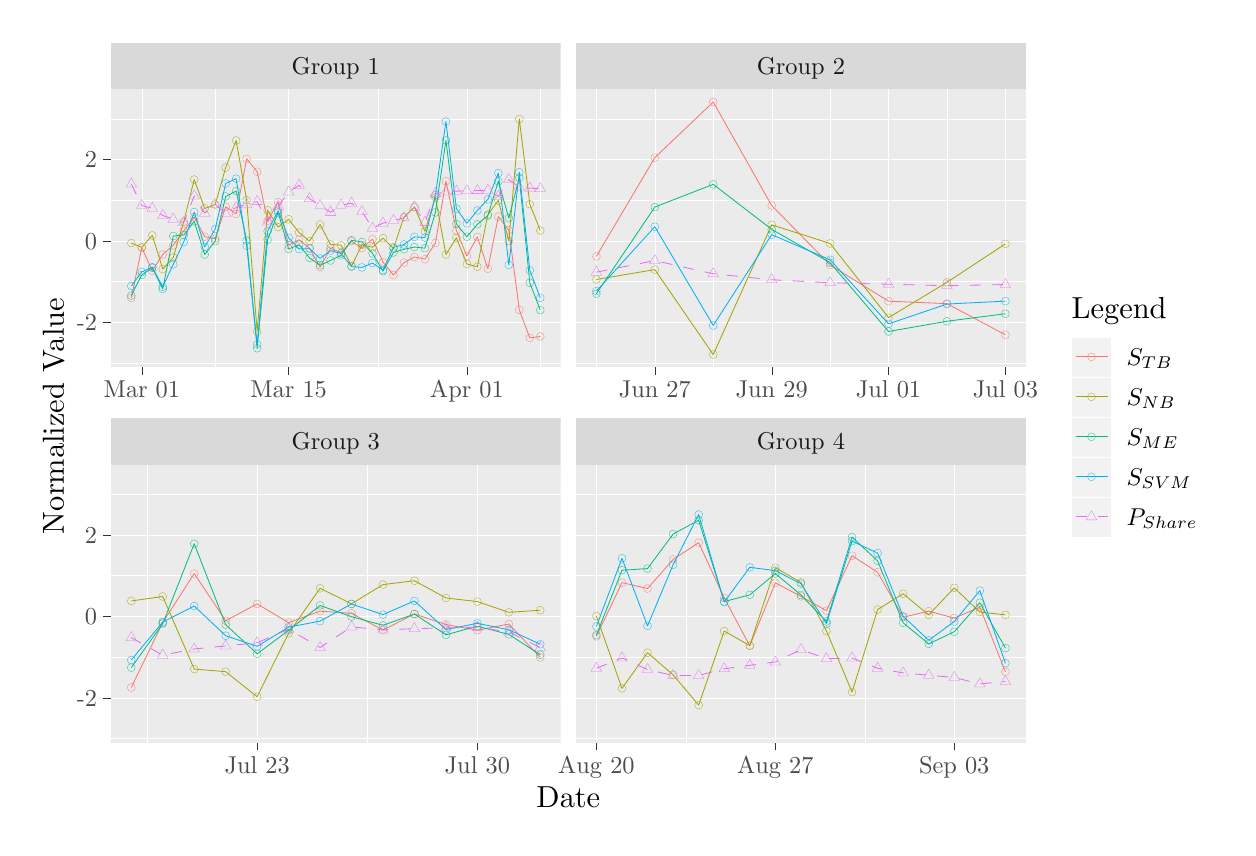
\begin{tikzpicture}[x=1pt,y=1pt]
\definecolor{fillColor}{RGB}{255,255,255}
\path[use as bounding box,fill=fillColor,fill opacity=0.00] (0,0) rectangle (433.62,289.08);
\begin{scope}
\path[clip] (  0.00,  0.00) rectangle (433.62,289.08);
\definecolor{drawColor}{RGB}{255,255,255}
\definecolor{fillColor}{RGB}{255,255,255}

\path[draw=drawColor,line width= 0.1pt,line join=round,line cap=round,fill=fillColor] (  0.00,  0.00) rectangle (433.62,289.08);
\end{scope}
\begin{scope}
\path[clip] ( 30.06,166.38) rectangle (192.62,266.77);
\definecolor{fillColor}{gray}{0.92}

\path[fill=fillColor] ( 30.06,166.38) rectangle (192.62,266.77);
\definecolor{drawColor}{RGB}{255,255,255}

\path[draw=drawColor,line width= 0.1pt,line join=round] ( 30.06,167.90) --
	(192.62,167.90);

\path[draw=drawColor,line width= 0.1pt,line join=round] ( 30.06,197.33) --
	(192.62,197.33);

\path[draw=drawColor,line width= 0.1pt,line join=round] ( 30.06,226.76) --
	(192.62,226.76);

\path[draw=drawColor,line width= 0.1pt,line join=round] ( 30.06,256.20) --
	(192.62,256.20);

\path[draw=drawColor,line width= 0.1pt,line join=round] ( 67.76,166.38) --
	( 67.76,266.77);

\path[draw=drawColor,line width= 0.1pt,line join=round] (126.50,166.38) --
	(126.50,266.77);

\path[draw=drawColor,line width= 0.1pt,line join=round] (185.23,166.38) --
	(185.23,266.77);

\path[draw=drawColor,line width= 0.1pt,line join=round] ( 30.06,182.62) --
	(192.62,182.62);

\path[draw=drawColor,line width= 0.1pt,line join=round] ( 30.06,212.05) --
	(192.62,212.05);

\path[draw=drawColor,line width= 0.1pt,line join=round] ( 30.06,241.48) --
	(192.62,241.48);

\path[draw=drawColor,line width= 0.1pt,line join=round] ( 41.23,166.38) --
	( 41.23,266.77);

\path[draw=drawColor,line width= 0.1pt,line join=round] ( 94.29,166.38) --
	( 94.29,266.77);

\path[draw=drawColor,line width= 0.1pt,line join=round] (158.71,166.38) --
	(158.71,266.77);
\definecolor{drawColor}{RGB}{248,118,109}

\path[draw=drawColor,line width= 0.3pt,line join=round] ( 37.44,191.42) --
	( 41.23,209.59) --
	( 45.02,201.23) --
	( 48.81,207.13) --
	( 52.60,210.44) --
	( 56.39,215.63) --
	( 60.18,220.64) --
	( 63.97,213.55) --
	( 67.76,212.85) --
	( 71.55,224.35) --
	( 75.34,221.79) --
	( 79.13,241.68) --
	( 82.92,237.02) --
	( 86.71,219.35) --
	( 90.50,226.01) --
	( 94.29,210.55) --
	( 98.08,212.45) --
	(101.86,209.41) --
	(105.65,202.53) --
	(109.44,209.36) --
	(113.23,207.69) --
	(117.02,211.93) --
	(120.81,209.45) --
	(124.60,212.65) --
	(128.39,204.37) --
	(132.18,199.69) --
	(135.97,204.19) --
	(139.76,206.22) --
	(143.55,205.44) --
	(147.34,211.27) --
	(151.13,233.62) --
	(154.92,215.74) --
	(158.71,206.58) --
	(162.49,213.48) --
	(166.28,201.98) --
	(170.07,220.82) --
	(173.86,215.92) --
	(177.65,187.12) --
	(181.44,176.98) --
	(185.23,177.49);
\definecolor{drawColor}{RGB}{163,165,0}

\path[draw=drawColor,line width= 0.3pt,line join=round] ( 37.44,211.24) --
	( 41.23,209.69) --
	( 45.02,214.02) --
	( 48.81,201.84) --
	( 52.60,206.00) --
	( 56.39,218.98) --
	( 60.18,234.20) --
	( 63.97,223.75) --
	( 67.76,225.16) --
	( 71.55,238.53) --
	( 75.34,248.32) --
	( 79.13,226.73) --
	( 82.92,179.35) --
	( 86.71,223.09) --
	( 90.50,217.02) --
	( 94.29,219.83) --
	( 98.08,215.07) --
	(101.86,211.96) --
	(105.65,217.97) --
	(109.44,210.75) --
	(113.23,210.51) --
	(117.02,202.91) --
	(120.81,210.58) --
	(124.60,209.75) --
	(128.39,213.02) --
	(132.18,209.29) --
	(135.97,220.67) --
	(139.76,224.24) --
	(143.55,215.49) --
	(147.34,227.75) --
	(151.13,207.11) --
	(154.92,213.14) --
	(158.71,203.68) --
	(162.49,202.70) --
	(166.28,221.50) --
	(170.07,226.65) --
	(173.86,211.98) --
	(177.65,256.08) --
	(181.44,225.32) --
	(185.23,215.78);
\definecolor{drawColor}{RGB}{0,191,125}

\path[draw=drawColor,line width= 0.3pt,line join=round] ( 37.44,192.30) --
	( 41.23,199.71) --
	( 45.02,202.31) --
	( 48.81,194.66) --
	( 52.60,213.79) --
	( 56.39,214.16) --
	( 60.18,219.11) --
	( 63.97,207.11) --
	( 67.76,211.96) --
	( 71.55,228.09) --
	( 75.34,230.04) --
	( 79.13,212.13) --
	( 82.92,173.23) --
	( 86.71,212.46) --
	( 90.50,222.32) --
	( 94.29,209.11) --
	( 98.08,210.64) --
	(101.86,205.85) --
	(105.65,203.25) --
	(109.44,204.96) --
	(113.23,206.82) --
	(117.02,212.27) --
	(120.81,211.64) --
	(124.60,207.52) --
	(128.39,201.10) --
	(132.18,207.85) --
	(135.97,209.00) --
	(139.76,209.79) --
	(143.55,209.41) --
	(147.34,222.33) --
	(151.13,248.34) --
	(154.92,218.15) --
	(158.71,213.53) --
	(162.49,218.03) --
	(166.28,221.16) --
	(170.07,233.59) --
	(173.86,220.26) --
	(177.65,234.81) --
	(181.44,196.90) --
	(185.23,187.02);
\definecolor{drawColor}{RGB}{0,176,246}

\path[draw=drawColor,line width= 0.3pt,line join=round] ( 37.44,195.74) --
	( 41.23,200.80) --
	( 45.02,202.52) --
	( 48.81,195.45) --
	( 52.60,203.54) --
	( 56.39,211.61) --
	( 60.18,222.45) --
	( 63.97,209.85) --
	( 67.76,216.32) --
	( 71.55,232.78) --
	( 75.34,234.51) --
	( 79.13,210.28) --
	( 82.92,174.63) --
	( 86.71,215.53) --
	( 90.50,222.90) --
	( 94.29,213.16) --
	( 98.08,209.08) --
	(101.86,209.24) --
	(105.65,205.70) --
	(109.44,208.51) --
	(113.23,207.47) --
	(117.02,202.74) --
	(120.81,202.44) --
	(124.60,204.02) --
	(128.39,201.49) --
	(132.18,209.68) --
	(135.97,210.72) --
	(139.76,213.48) --
	(143.55,213.25) --
	(147.34,228.56) --
	(151.13,255.15) --
	(154.92,223.70) --
	(158.71,218.38) --
	(162.49,223.03) --
	(166.28,227.02) --
	(170.07,236.52) --
	(173.86,203.34) --
	(177.65,236.85) --
	(181.44,201.39) --
	(185.23,191.44);
\definecolor{drawColor}{RGB}{231,107,243}

\path[draw=drawColor,line width= 0.3pt,dash pattern=on 4pt off 4pt ,line join=round] ( 37.44,232.59) --
	( 41.23,224.81) --
	( 45.02,223.80) --
	( 48.81,221.20) --
	( 52.60,219.91) --
	( 56.39,218.61) --
	( 60.18,228.27) --
	( 63.97,222.07) --
	( 67.76,225.24) --
	( 71.55,221.92) --
	( 75.34,224.09) --
	( 79.13,225.17) --
	( 82.92,226.25) --
	( 86.71,218.90) --
	( 90.50,224.52) --
	( 94.29,229.71) --
	( 98.08,232.16) --
	(101.86,227.26) --
	(105.65,224.81) --
	(109.44,222.36) --
	(113.23,224.95) --
	(117.02,225.67) --
	(120.81,222.65) --
	(124.60,216.59) --
	(128.39,218.46) --
	(132.18,219.40) --
	(135.97,220.34) --
	(139.76,224.23) --
	(143.55,218.75) --
	(147.34,229.13) --
	(151.13,229.71) --
	(154.92,230.00) --
	(158.71,230.14) --
	(162.49,230.22) --
	(166.28,230.29) --
	(170.07,228.12) --
	(173.86,234.18) --
	(177.65,231.44) --
	(181.44,231.08) --
	(185.23,230.90);
\definecolor{drawColor}{RGB}{248,118,109}

\path[draw=drawColor,line width= 0.1pt,line join=round,line cap=round] ( 37.44,191.42) circle (  1.43);

\path[draw=drawColor,line width= 0.1pt,line join=round,line cap=round] ( 41.23,209.59) circle (  1.43);

\path[draw=drawColor,line width= 0.1pt,line join=round,line cap=round] ( 45.02,201.23) circle (  1.43);

\path[draw=drawColor,line width= 0.1pt,line join=round,line cap=round] ( 48.81,207.13) circle (  1.43);

\path[draw=drawColor,line width= 0.1pt,line join=round,line cap=round] ( 52.60,210.44) circle (  1.43);

\path[draw=drawColor,line width= 0.1pt,line join=round,line cap=round] ( 56.39,215.63) circle (  1.43);

\path[draw=drawColor,line width= 0.1pt,line join=round,line cap=round] ( 60.18,220.64) circle (  1.43);

\path[draw=drawColor,line width= 0.1pt,line join=round,line cap=round] ( 63.97,213.55) circle (  1.43);

\path[draw=drawColor,line width= 0.1pt,line join=round,line cap=round] ( 67.76,212.85) circle (  1.43);

\path[draw=drawColor,line width= 0.1pt,line join=round,line cap=round] ( 71.55,224.35) circle (  1.43);

\path[draw=drawColor,line width= 0.1pt,line join=round,line cap=round] ( 75.34,221.79) circle (  1.43);

\path[draw=drawColor,line width= 0.1pt,line join=round,line cap=round] ( 79.13,241.68) circle (  1.43);

\path[draw=drawColor,line width= 0.1pt,line join=round,line cap=round] ( 82.92,237.02) circle (  1.43);

\path[draw=drawColor,line width= 0.1pt,line join=round,line cap=round] ( 86.71,219.35) circle (  1.43);

\path[draw=drawColor,line width= 0.1pt,line join=round,line cap=round] ( 90.50,226.01) circle (  1.43);

\path[draw=drawColor,line width= 0.1pt,line join=round,line cap=round] ( 94.29,210.55) circle (  1.43);

\path[draw=drawColor,line width= 0.1pt,line join=round,line cap=round] ( 98.08,212.45) circle (  1.43);

\path[draw=drawColor,line width= 0.1pt,line join=round,line cap=round] (101.86,209.41) circle (  1.43);

\path[draw=drawColor,line width= 0.1pt,line join=round,line cap=round] (105.65,202.53) circle (  1.43);

\path[draw=drawColor,line width= 0.1pt,line join=round,line cap=round] (109.44,209.36) circle (  1.43);

\path[draw=drawColor,line width= 0.1pt,line join=round,line cap=round] (113.23,207.69) circle (  1.43);

\path[draw=drawColor,line width= 0.1pt,line join=round,line cap=round] (117.02,211.93) circle (  1.43);

\path[draw=drawColor,line width= 0.1pt,line join=round,line cap=round] (120.81,209.45) circle (  1.43);

\path[draw=drawColor,line width= 0.1pt,line join=round,line cap=round] (124.60,212.65) circle (  1.43);

\path[draw=drawColor,line width= 0.1pt,line join=round,line cap=round] (128.39,204.37) circle (  1.43);

\path[draw=drawColor,line width= 0.1pt,line join=round,line cap=round] (132.18,199.69) circle (  1.43);

\path[draw=drawColor,line width= 0.1pt,line join=round,line cap=round] (135.97,204.19) circle (  1.43);

\path[draw=drawColor,line width= 0.1pt,line join=round,line cap=round] (139.76,206.22) circle (  1.43);

\path[draw=drawColor,line width= 0.1pt,line join=round,line cap=round] (143.55,205.44) circle (  1.43);

\path[draw=drawColor,line width= 0.1pt,line join=round,line cap=round] (147.34,211.27) circle (  1.43);

\path[draw=drawColor,line width= 0.1pt,line join=round,line cap=round] (151.13,233.62) circle (  1.43);

\path[draw=drawColor,line width= 0.1pt,line join=round,line cap=round] (154.92,215.74) circle (  1.43);

\path[draw=drawColor,line width= 0.1pt,line join=round,line cap=round] (158.71,206.58) circle (  1.43);

\path[draw=drawColor,line width= 0.1pt,line join=round,line cap=round] (162.49,213.48) circle (  1.43);

\path[draw=drawColor,line width= 0.1pt,line join=round,line cap=round] (166.28,201.98) circle (  1.43);

\path[draw=drawColor,line width= 0.1pt,line join=round,line cap=round] (170.07,220.82) circle (  1.43);

\path[draw=drawColor,line width= 0.1pt,line join=round,line cap=round] (173.86,215.92) circle (  1.43);

\path[draw=drawColor,line width= 0.1pt,line join=round,line cap=round] (177.65,187.12) circle (  1.43);

\path[draw=drawColor,line width= 0.1pt,line join=round,line cap=round] (181.44,176.98) circle (  1.43);

\path[draw=drawColor,line width= 0.1pt,line join=round,line cap=round] (185.23,177.49) circle (  1.43);
\definecolor{drawColor}{RGB}{163,165,0}

\path[draw=drawColor,line width= 0.1pt,line join=round,line cap=round] ( 37.44,211.24) circle (  1.43);

\path[draw=drawColor,line width= 0.1pt,line join=round,line cap=round] ( 41.23,209.69) circle (  1.43);

\path[draw=drawColor,line width= 0.1pt,line join=round,line cap=round] ( 45.02,214.02) circle (  1.43);

\path[draw=drawColor,line width= 0.1pt,line join=round,line cap=round] ( 48.81,201.84) circle (  1.43);

\path[draw=drawColor,line width= 0.1pt,line join=round,line cap=round] ( 52.60,206.00) circle (  1.43);

\path[draw=drawColor,line width= 0.1pt,line join=round,line cap=round] ( 56.39,218.98) circle (  1.43);

\path[draw=drawColor,line width= 0.1pt,line join=round,line cap=round] ( 60.18,234.20) circle (  1.43);

\path[draw=drawColor,line width= 0.1pt,line join=round,line cap=round] ( 63.97,223.75) circle (  1.43);

\path[draw=drawColor,line width= 0.1pt,line join=round,line cap=round] ( 67.76,225.16) circle (  1.43);

\path[draw=drawColor,line width= 0.1pt,line join=round,line cap=round] ( 71.55,238.53) circle (  1.43);

\path[draw=drawColor,line width= 0.1pt,line join=round,line cap=round] ( 75.34,248.32) circle (  1.43);

\path[draw=drawColor,line width= 0.1pt,line join=round,line cap=round] ( 79.13,226.73) circle (  1.43);

\path[draw=drawColor,line width= 0.1pt,line join=round,line cap=round] ( 82.92,179.35) circle (  1.43);

\path[draw=drawColor,line width= 0.1pt,line join=round,line cap=round] ( 86.71,223.09) circle (  1.43);

\path[draw=drawColor,line width= 0.1pt,line join=round,line cap=round] ( 90.50,217.02) circle (  1.43);

\path[draw=drawColor,line width= 0.1pt,line join=round,line cap=round] ( 94.29,219.83) circle (  1.43);

\path[draw=drawColor,line width= 0.1pt,line join=round,line cap=round] ( 98.08,215.07) circle (  1.43);

\path[draw=drawColor,line width= 0.1pt,line join=round,line cap=round] (101.86,211.96) circle (  1.43);

\path[draw=drawColor,line width= 0.1pt,line join=round,line cap=round] (105.65,217.97) circle (  1.43);

\path[draw=drawColor,line width= 0.1pt,line join=round,line cap=round] (109.44,210.75) circle (  1.43);

\path[draw=drawColor,line width= 0.1pt,line join=round,line cap=round] (113.23,210.51) circle (  1.43);

\path[draw=drawColor,line width= 0.1pt,line join=round,line cap=round] (117.02,202.91) circle (  1.43);

\path[draw=drawColor,line width= 0.1pt,line join=round,line cap=round] (120.81,210.58) circle (  1.43);

\path[draw=drawColor,line width= 0.1pt,line join=round,line cap=round] (124.60,209.75) circle (  1.43);

\path[draw=drawColor,line width= 0.1pt,line join=round,line cap=round] (128.39,213.02) circle (  1.43);

\path[draw=drawColor,line width= 0.1pt,line join=round,line cap=round] (132.18,209.29) circle (  1.43);

\path[draw=drawColor,line width= 0.1pt,line join=round,line cap=round] (135.97,220.67) circle (  1.43);

\path[draw=drawColor,line width= 0.1pt,line join=round,line cap=round] (139.76,224.24) circle (  1.43);

\path[draw=drawColor,line width= 0.1pt,line join=round,line cap=round] (143.55,215.49) circle (  1.43);

\path[draw=drawColor,line width= 0.1pt,line join=round,line cap=round] (147.34,227.75) circle (  1.43);

\path[draw=drawColor,line width= 0.1pt,line join=round,line cap=round] (151.13,207.11) circle (  1.43);

\path[draw=drawColor,line width= 0.1pt,line join=round,line cap=round] (154.92,213.14) circle (  1.43);

\path[draw=drawColor,line width= 0.1pt,line join=round,line cap=round] (158.71,203.68) circle (  1.43);

\path[draw=drawColor,line width= 0.1pt,line join=round,line cap=round] (162.49,202.70) circle (  1.43);

\path[draw=drawColor,line width= 0.1pt,line join=round,line cap=round] (166.28,221.50) circle (  1.43);

\path[draw=drawColor,line width= 0.1pt,line join=round,line cap=round] (170.07,226.65) circle (  1.43);

\path[draw=drawColor,line width= 0.1pt,line join=round,line cap=round] (173.86,211.98) circle (  1.43);

\path[draw=drawColor,line width= 0.1pt,line join=round,line cap=round] (177.65,256.08) circle (  1.43);

\path[draw=drawColor,line width= 0.1pt,line join=round,line cap=round] (181.44,225.32) circle (  1.43);

\path[draw=drawColor,line width= 0.1pt,line join=round,line cap=round] (185.23,215.78) circle (  1.43);
\definecolor{drawColor}{RGB}{0,191,125}

\path[draw=drawColor,line width= 0.1pt,line join=round,line cap=round] ( 37.44,192.30) circle (  1.43);

\path[draw=drawColor,line width= 0.1pt,line join=round,line cap=round] ( 41.23,199.71) circle (  1.43);

\path[draw=drawColor,line width= 0.1pt,line join=round,line cap=round] ( 45.02,202.31) circle (  1.43);

\path[draw=drawColor,line width= 0.1pt,line join=round,line cap=round] ( 48.81,194.66) circle (  1.43);

\path[draw=drawColor,line width= 0.1pt,line join=round,line cap=round] ( 52.60,213.79) circle (  1.43);

\path[draw=drawColor,line width= 0.1pt,line join=round,line cap=round] ( 56.39,214.16) circle (  1.43);

\path[draw=drawColor,line width= 0.1pt,line join=round,line cap=round] ( 60.18,219.11) circle (  1.43);

\path[draw=drawColor,line width= 0.1pt,line join=round,line cap=round] ( 63.97,207.11) circle (  1.43);

\path[draw=drawColor,line width= 0.1pt,line join=round,line cap=round] ( 67.76,211.96) circle (  1.43);

\path[draw=drawColor,line width= 0.1pt,line join=round,line cap=round] ( 71.55,228.09) circle (  1.43);

\path[draw=drawColor,line width= 0.1pt,line join=round,line cap=round] ( 75.34,230.04) circle (  1.43);

\path[draw=drawColor,line width= 0.1pt,line join=round,line cap=round] ( 79.13,212.13) circle (  1.43);

\path[draw=drawColor,line width= 0.1pt,line join=round,line cap=round] ( 82.92,173.23) circle (  1.43);

\path[draw=drawColor,line width= 0.1pt,line join=round,line cap=round] ( 86.71,212.46) circle (  1.43);

\path[draw=drawColor,line width= 0.1pt,line join=round,line cap=round] ( 90.50,222.32) circle (  1.43);

\path[draw=drawColor,line width= 0.1pt,line join=round,line cap=round] ( 94.29,209.11) circle (  1.43);

\path[draw=drawColor,line width= 0.1pt,line join=round,line cap=round] ( 98.08,210.64) circle (  1.43);

\path[draw=drawColor,line width= 0.1pt,line join=round,line cap=round] (101.86,205.85) circle (  1.43);

\path[draw=drawColor,line width= 0.1pt,line join=round,line cap=round] (105.65,203.25) circle (  1.43);

\path[draw=drawColor,line width= 0.1pt,line join=round,line cap=round] (109.44,204.96) circle (  1.43);

\path[draw=drawColor,line width= 0.1pt,line join=round,line cap=round] (113.23,206.82) circle (  1.43);

\path[draw=drawColor,line width= 0.1pt,line join=round,line cap=round] (117.02,212.27) circle (  1.43);

\path[draw=drawColor,line width= 0.1pt,line join=round,line cap=round] (120.81,211.64) circle (  1.43);

\path[draw=drawColor,line width= 0.1pt,line join=round,line cap=round] (124.60,207.52) circle (  1.43);

\path[draw=drawColor,line width= 0.1pt,line join=round,line cap=round] (128.39,201.10) circle (  1.43);

\path[draw=drawColor,line width= 0.1pt,line join=round,line cap=round] (132.18,207.85) circle (  1.43);

\path[draw=drawColor,line width= 0.1pt,line join=round,line cap=round] (135.97,209.00) circle (  1.43);

\path[draw=drawColor,line width= 0.1pt,line join=round,line cap=round] (139.76,209.79) circle (  1.43);

\path[draw=drawColor,line width= 0.1pt,line join=round,line cap=round] (143.55,209.41) circle (  1.43);

\path[draw=drawColor,line width= 0.1pt,line join=round,line cap=round] (147.34,222.33) circle (  1.43);

\path[draw=drawColor,line width= 0.1pt,line join=round,line cap=round] (151.13,248.34) circle (  1.43);

\path[draw=drawColor,line width= 0.1pt,line join=round,line cap=round] (154.92,218.15) circle (  1.43);

\path[draw=drawColor,line width= 0.1pt,line join=round,line cap=round] (158.71,213.53) circle (  1.43);

\path[draw=drawColor,line width= 0.1pt,line join=round,line cap=round] (162.49,218.03) circle (  1.43);

\path[draw=drawColor,line width= 0.1pt,line join=round,line cap=round] (166.28,221.16) circle (  1.43);

\path[draw=drawColor,line width= 0.1pt,line join=round,line cap=round] (170.07,233.59) circle (  1.43);

\path[draw=drawColor,line width= 0.1pt,line join=round,line cap=round] (173.86,220.26) circle (  1.43);

\path[draw=drawColor,line width= 0.1pt,line join=round,line cap=round] (177.65,234.81) circle (  1.43);

\path[draw=drawColor,line width= 0.1pt,line join=round,line cap=round] (181.44,196.90) circle (  1.43);

\path[draw=drawColor,line width= 0.1pt,line join=round,line cap=round] (185.23,187.02) circle (  1.43);
\definecolor{drawColor}{RGB}{0,176,246}

\path[draw=drawColor,line width= 0.1pt,line join=round,line cap=round] ( 37.44,195.74) circle (  1.43);

\path[draw=drawColor,line width= 0.1pt,line join=round,line cap=round] ( 41.23,200.80) circle (  1.43);

\path[draw=drawColor,line width= 0.1pt,line join=round,line cap=round] ( 45.02,202.52) circle (  1.43);

\path[draw=drawColor,line width= 0.1pt,line join=round,line cap=round] ( 48.81,195.45) circle (  1.43);

\path[draw=drawColor,line width= 0.1pt,line join=round,line cap=round] ( 52.60,203.54) circle (  1.43);

\path[draw=drawColor,line width= 0.1pt,line join=round,line cap=round] ( 56.39,211.61) circle (  1.43);

\path[draw=drawColor,line width= 0.1pt,line join=round,line cap=round] ( 60.18,222.45) circle (  1.43);

\path[draw=drawColor,line width= 0.1pt,line join=round,line cap=round] ( 63.97,209.85) circle (  1.43);

\path[draw=drawColor,line width= 0.1pt,line join=round,line cap=round] ( 67.76,216.32) circle (  1.43);

\path[draw=drawColor,line width= 0.1pt,line join=round,line cap=round] ( 71.55,232.78) circle (  1.43);

\path[draw=drawColor,line width= 0.1pt,line join=round,line cap=round] ( 75.34,234.51) circle (  1.43);

\path[draw=drawColor,line width= 0.1pt,line join=round,line cap=round] ( 79.13,210.28) circle (  1.43);

\path[draw=drawColor,line width= 0.1pt,line join=round,line cap=round] ( 82.92,174.63) circle (  1.43);

\path[draw=drawColor,line width= 0.1pt,line join=round,line cap=round] ( 86.71,215.53) circle (  1.43);

\path[draw=drawColor,line width= 0.1pt,line join=round,line cap=round] ( 90.50,222.90) circle (  1.43);

\path[draw=drawColor,line width= 0.1pt,line join=round,line cap=round] ( 94.29,213.16) circle (  1.43);

\path[draw=drawColor,line width= 0.1pt,line join=round,line cap=round] ( 98.08,209.08) circle (  1.43);

\path[draw=drawColor,line width= 0.1pt,line join=round,line cap=round] (101.86,209.24) circle (  1.43);

\path[draw=drawColor,line width= 0.1pt,line join=round,line cap=round] (105.65,205.70) circle (  1.43);

\path[draw=drawColor,line width= 0.1pt,line join=round,line cap=round] (109.44,208.51) circle (  1.43);

\path[draw=drawColor,line width= 0.1pt,line join=round,line cap=round] (113.23,207.47) circle (  1.43);

\path[draw=drawColor,line width= 0.1pt,line join=round,line cap=round] (117.02,202.74) circle (  1.43);

\path[draw=drawColor,line width= 0.1pt,line join=round,line cap=round] (120.81,202.44) circle (  1.43);

\path[draw=drawColor,line width= 0.1pt,line join=round,line cap=round] (124.60,204.02) circle (  1.43);

\path[draw=drawColor,line width= 0.1pt,line join=round,line cap=round] (128.39,201.49) circle (  1.43);

\path[draw=drawColor,line width= 0.1pt,line join=round,line cap=round] (132.18,209.68) circle (  1.43);

\path[draw=drawColor,line width= 0.1pt,line join=round,line cap=round] (135.97,210.72) circle (  1.43);

\path[draw=drawColor,line width= 0.1pt,line join=round,line cap=round] (139.76,213.48) circle (  1.43);

\path[draw=drawColor,line width= 0.1pt,line join=round,line cap=round] (143.55,213.25) circle (  1.43);

\path[draw=drawColor,line width= 0.1pt,line join=round,line cap=round] (147.34,228.56) circle (  1.43);

\path[draw=drawColor,line width= 0.1pt,line join=round,line cap=round] (151.13,255.15) circle (  1.43);

\path[draw=drawColor,line width= 0.1pt,line join=round,line cap=round] (154.92,223.70) circle (  1.43);

\path[draw=drawColor,line width= 0.1pt,line join=round,line cap=round] (158.71,218.38) circle (  1.43);

\path[draw=drawColor,line width= 0.1pt,line join=round,line cap=round] (162.49,223.03) circle (  1.43);

\path[draw=drawColor,line width= 0.1pt,line join=round,line cap=round] (166.28,227.02) circle (  1.43);

\path[draw=drawColor,line width= 0.1pt,line join=round,line cap=round] (170.07,236.52) circle (  1.43);

\path[draw=drawColor,line width= 0.1pt,line join=round,line cap=round] (173.86,203.34) circle (  1.43);

\path[draw=drawColor,line width= 0.1pt,line join=round,line cap=round] (177.65,236.85) circle (  1.43);

\path[draw=drawColor,line width= 0.1pt,line join=round,line cap=round] (181.44,201.39) circle (  1.43);

\path[draw=drawColor,line width= 0.1pt,line join=round,line cap=round] (185.23,191.44) circle (  1.43);
\definecolor{drawColor}{RGB}{231,107,243}

\path[draw=drawColor,line width= 0.1pt,line join=round,line cap=round] ( 37.44,234.81) --
	( 39.37,231.49) --
	( 35.52,231.49) --
	( 37.44,234.81);

\path[draw=drawColor,line width= 0.1pt,line join=round,line cap=round] ( 41.23,227.03) --
	( 43.16,223.70) --
	( 39.31,223.70) --
	( 41.23,227.03);

\path[draw=drawColor,line width= 0.1pt,line join=round,line cap=round] ( 45.02,226.02) --
	( 46.94,222.69) --
	( 43.10,222.69) --
	( 45.02,226.02);

\path[draw=drawColor,line width= 0.1pt,line join=round,line cap=round] ( 48.81,223.42) --
	( 50.73,220.09) --
	( 46.89,220.09) --
	( 48.81,223.42);

\path[draw=drawColor,line width= 0.1pt,line join=round,line cap=round] ( 52.60,222.12) --
	( 54.52,218.80) --
	( 50.68,218.80) --
	( 52.60,222.12);

\path[draw=drawColor,line width= 0.1pt,line join=round,line cap=round] ( 56.39,220.83) --
	( 58.31,217.50) --
	( 54.47,217.50) --
	( 56.39,220.83);

\path[draw=drawColor,line width= 0.1pt,line join=round,line cap=round] ( 60.18,230.49) --
	( 62.10,227.16) --
	( 58.26,227.16) --
	( 60.18,230.49);

\path[draw=drawColor,line width= 0.1pt,line join=round,line cap=round] ( 63.97,224.29) --
	( 65.89,220.96) --
	( 62.05,220.96) --
	( 63.97,224.29);

\path[draw=drawColor,line width= 0.1pt,line join=round,line cap=round] ( 67.76,227.46) --
	( 69.68,224.13) --
	( 65.84,224.13) --
	( 67.76,227.46);

\path[draw=drawColor,line width= 0.1pt,line join=round,line cap=round] ( 71.55,224.14) --
	( 73.47,220.82) --
	( 69.63,220.82) --
	( 71.55,224.14);

\path[draw=drawColor,line width= 0.1pt,line join=round,line cap=round] ( 75.34,226.31) --
	( 77.26,222.98) --
	( 73.42,222.98) --
	( 75.34,226.31);

\path[draw=drawColor,line width= 0.1pt,line join=round,line cap=round] ( 79.13,227.39) --
	( 81.05,224.06) --
	( 77.21,224.06) --
	( 79.13,227.39);

\path[draw=drawColor,line width= 0.1pt,line join=round,line cap=round] ( 82.92,228.47) --
	( 84.84,225.14) --
	( 81.00,225.14) --
	( 82.92,228.47);

\path[draw=drawColor,line width= 0.1pt,line join=round,line cap=round] ( 86.71,221.12) --
	( 88.63,217.79) --
	( 84.79,217.79) --
	( 86.71,221.12);

\path[draw=drawColor,line width= 0.1pt,line join=round,line cap=round] ( 90.50,226.74) --
	( 92.42,223.41) --
	( 88.57,223.41) --
	( 90.50,226.74);

\path[draw=drawColor,line width= 0.1pt,line join=round,line cap=round] ( 94.29,231.93) --
	( 96.21,228.60) --
	( 92.36,228.60) --
	( 94.29,231.93);

\path[draw=drawColor,line width= 0.1pt,line join=round,line cap=round] ( 98.08,234.38) --
	(100.00,231.05) --
	( 96.15,231.05) --
	( 98.08,234.38);

\path[draw=drawColor,line width= 0.1pt,line join=round,line cap=round] (101.86,229.48) --
	(103.79,226.15) --
	( 99.94,226.15) --
	(101.86,229.48);

\path[draw=drawColor,line width= 0.1pt,line join=round,line cap=round] (105.65,227.03) --
	(107.58,223.70) --
	(103.73,223.70) --
	(105.65,227.03);

\path[draw=drawColor,line width= 0.1pt,line join=round,line cap=round] (109.44,224.58) --
	(111.36,221.25) --
	(107.52,221.25) --
	(109.44,224.58);

\path[draw=drawColor,line width= 0.1pt,line join=round,line cap=round] (113.23,227.17) --
	(115.15,223.84) --
	(111.31,223.84) --
	(113.23,227.17);

\path[draw=drawColor,line width= 0.1pt,line join=round,line cap=round] (117.02,227.89) --
	(118.94,224.56) --
	(115.10,224.56) --
	(117.02,227.89);

\path[draw=drawColor,line width= 0.1pt,line join=round,line cap=round] (120.81,224.86) --
	(122.73,221.54) --
	(118.89,221.54) --
	(120.81,224.86);

\path[draw=drawColor,line width= 0.1pt,line join=round,line cap=round] (124.60,218.81) --
	(126.52,215.48) --
	(122.68,215.48) --
	(124.60,218.81);

\path[draw=drawColor,line width= 0.1pt,line join=round,line cap=round] (128.39,220.68) --
	(130.31,217.35) --
	(126.47,217.35) --
	(128.39,220.68);

\path[draw=drawColor,line width= 0.1pt,line join=round,line cap=round] (132.18,221.62) --
	(134.10,218.29) --
	(130.26,218.29) --
	(132.18,221.62);

\path[draw=drawColor,line width= 0.1pt,line join=round,line cap=round] (135.97,222.56) --
	(137.89,219.23) --
	(134.05,219.23) --
	(135.97,222.56);

\path[draw=drawColor,line width= 0.1pt,line join=round,line cap=round] (139.76,226.45) --
	(141.68,223.12) --
	(137.84,223.12) --
	(139.76,226.45);

\path[draw=drawColor,line width= 0.1pt,line join=round,line cap=round] (143.55,220.97) --
	(145.47,217.64) --
	(141.63,217.64) --
	(143.55,220.97);

\path[draw=drawColor,line width= 0.1pt,line join=round,line cap=round] (147.34,231.35) --
	(149.26,228.02) --
	(145.42,228.02) --
	(147.34,231.35);

\path[draw=drawColor,line width= 0.1pt,line join=round,line cap=round] (151.13,231.93) --
	(153.05,228.60) --
	(149.21,228.60) --
	(151.13,231.93);

\path[draw=drawColor,line width= 0.1pt,line join=round,line cap=round] (154.92,232.22) --
	(156.84,228.89) --
	(152.99,228.89) --
	(154.92,232.22);

\path[draw=drawColor,line width= 0.1pt,line join=round,line cap=round] (158.71,232.36) --
	(160.63,229.03) --
	(156.78,229.03) --
	(158.71,232.36);

\path[draw=drawColor,line width= 0.1pt,line join=round,line cap=round] (162.49,232.43) --
	(164.42,229.11) --
	(160.57,229.11) --
	(162.49,232.43);

\path[draw=drawColor,line width= 0.1pt,line join=round,line cap=round] (166.28,232.51) --
	(168.21,229.18) --
	(164.36,229.18) --
	(166.28,232.51);

\path[draw=drawColor,line width= 0.1pt,line join=round,line cap=round] (170.07,230.34) --
	(171.99,227.02) --
	(168.15,227.02) --
	(170.07,230.34);

\path[draw=drawColor,line width= 0.1pt,line join=round,line cap=round] (173.86,236.40) --
	(175.78,233.07) --
	(171.94,233.07) --
	(173.86,236.40);

\path[draw=drawColor,line width= 0.1pt,line join=round,line cap=round] (177.65,233.66) --
	(179.57,230.33) --
	(175.73,230.33) --
	(177.65,233.66);

\path[draw=drawColor,line width= 0.1pt,line join=round,line cap=round] (181.44,233.30) --
	(183.36,229.97) --
	(179.52,229.97) --
	(181.44,233.30);

\path[draw=drawColor,line width= 0.1pt,line join=round,line cap=round] (185.23,233.12) --
	(187.15,229.79) --
	(183.31,229.79) --
	(185.23,233.12);
\end{scope}
\begin{scope}
\path[clip] ( 30.06, 30.73) rectangle (192.62,131.12);
\definecolor{fillColor}{gray}{0.92}

\path[fill=fillColor] ( 30.06, 30.73) rectangle (192.62,131.12);
\definecolor{drawColor}{RGB}{255,255,255}

\path[draw=drawColor,line width= 0.1pt,line join=round] ( 30.06, 32.25) --
	(192.62, 32.25);

\path[draw=drawColor,line width= 0.1pt,line join=round] ( 30.06, 61.68) --
	(192.62, 61.68);

\path[draw=drawColor,line width= 0.1pt,line join=round] ( 30.06, 91.11) --
	(192.62, 91.11);

\path[draw=drawColor,line width= 0.1pt,line join=round] ( 30.06,120.54) --
	(192.62,120.54);

\path[draw=drawColor,line width= 0.1pt,line join=round] ( 43.13, 30.73) --
	( 43.13,131.12);

\path[draw=drawColor,line width= 0.1pt,line join=round] (122.71, 30.73) --
	(122.71,131.12);

\path[draw=drawColor,line width= 0.1pt,line join=round] ( 30.06, 46.96) --
	(192.62, 46.96);

\path[draw=drawColor,line width= 0.1pt,line join=round] ( 30.06, 76.39) --
	(192.62, 76.39);

\path[draw=drawColor,line width= 0.1pt,line join=round] ( 30.06,105.83) --
	(192.62,105.83);

\path[draw=drawColor,line width= 0.1pt,line join=round] ( 82.92, 30.73) --
	( 82.92,131.12);

\path[draw=drawColor,line width= 0.1pt,line join=round] (162.49, 30.73) --
	(162.49,131.12);
\definecolor{drawColor}{RGB}{248,118,109}

\path[draw=drawColor,line width= 0.3pt,line join=round] ( 37.44, 50.67) --
	( 48.81, 74.13) --
	( 60.18, 91.82) --
	( 71.55, 74.77) --
	( 82.92, 80.87) --
	( 94.29, 74.09) --
	(105.65, 78.23) --
	(117.02, 77.48) --
	(128.39, 71.40) --
	(139.76, 77.22) --
	(151.13, 73.40) --
	(162.49, 71.34) --
	(173.86, 73.59) --
	(185.23, 61.53);
\definecolor{drawColor}{RGB}{163,165,0}

\path[draw=drawColor,line width= 0.3pt,line join=round] ( 37.44, 81.92) --
	( 48.81, 83.54) --
	( 60.18, 57.31) --
	( 71.55, 56.36) --
	( 82.92, 47.30) --
	( 94.29, 70.25) --
	(105.65, 86.50) --
	(117.02, 80.89) --
	(128.39, 87.84) --
	(139.76, 89.23) --
	(151.13, 83.01) --
	(162.49, 81.70) --
	(173.86, 77.82) --
	(185.23, 78.57);
\definecolor{drawColor}{RGB}{0,191,125}

\path[draw=drawColor,line width= 0.3pt,line join=round] ( 37.44, 57.82) --
	( 48.81, 73.72) --
	( 60.18,102.60) --
	( 71.55, 73.35) --
	( 82.92, 62.82) --
	( 94.29, 71.30) --
	(105.65, 80.29) --
	(117.02, 76.23) --
	(128.39, 73.12) --
	(139.76, 77.20) --
	(151.13, 69.68) --
	(162.49, 72.82) --
	(173.86, 69.84) --
	(185.23, 62.49);
\definecolor{drawColor}{RGB}{0,176,246}

\path[draw=drawColor,line width= 0.3pt,line join=round] ( 37.44, 60.59) --
	( 48.81, 74.31) --
	( 60.18, 80.08) --
	( 71.55, 69.36) --
	( 82.92, 65.53) --
	( 94.29, 72.46) --
	(105.65, 74.63) --
	(117.02, 80.82) --
	(128.39, 76.99) --
	(139.76, 81.94) --
	(151.13, 71.59) --
	(162.49, 73.84) --
	(173.86, 71.51) --
	(185.23, 66.29);
\definecolor{drawColor}{RGB}{231,107,243}

\path[draw=drawColor,line width= 0.3pt,dash pattern=on 4pt off 4pt ,line join=round] ( 37.44, 68.68) --
	( 48.81, 62.34) --
	( 60.18, 64.57) --
	( 71.55, 65.69) --
	( 82.92, 66.81) --
	( 94.29, 71.71) --
	(105.65, 65.08) --
	(117.02, 72.57) --
	(128.39, 71.42) --
	(139.76, 71.92) --
	(151.13, 72.18) --
	(162.49, 72.43) --
	(173.86, 70.70) --
	(185.23, 65.08);
\definecolor{drawColor}{RGB}{248,118,109}

\path[draw=drawColor,line width= 0.1pt,line join=round,line cap=round] ( 37.44, 50.67) circle (  1.43);

\path[draw=drawColor,line width= 0.1pt,line join=round,line cap=round] ( 48.81, 74.13) circle (  1.43);

\path[draw=drawColor,line width= 0.1pt,line join=round,line cap=round] ( 60.18, 91.82) circle (  1.43);

\path[draw=drawColor,line width= 0.1pt,line join=round,line cap=round] ( 71.55, 74.77) circle (  1.43);

\path[draw=drawColor,line width= 0.1pt,line join=round,line cap=round] ( 82.92, 80.87) circle (  1.43);

\path[draw=drawColor,line width= 0.1pt,line join=round,line cap=round] ( 94.29, 74.09) circle (  1.43);

\path[draw=drawColor,line width= 0.1pt,line join=round,line cap=round] (105.65, 78.23) circle (  1.43);

\path[draw=drawColor,line width= 0.1pt,line join=round,line cap=round] (117.02, 77.48) circle (  1.43);

\path[draw=drawColor,line width= 0.1pt,line join=round,line cap=round] (128.39, 71.40) circle (  1.43);

\path[draw=drawColor,line width= 0.1pt,line join=round,line cap=round] (139.76, 77.22) circle (  1.43);

\path[draw=drawColor,line width= 0.1pt,line join=round,line cap=round] (151.13, 73.40) circle (  1.43);

\path[draw=drawColor,line width= 0.1pt,line join=round,line cap=round] (162.49, 71.34) circle (  1.43);

\path[draw=drawColor,line width= 0.1pt,line join=round,line cap=round] (173.86, 73.59) circle (  1.43);

\path[draw=drawColor,line width= 0.1pt,line join=round,line cap=round] (185.23, 61.53) circle (  1.43);
\definecolor{drawColor}{RGB}{163,165,0}

\path[draw=drawColor,line width= 0.1pt,line join=round,line cap=round] ( 37.44, 81.92) circle (  1.43);

\path[draw=drawColor,line width= 0.1pt,line join=round,line cap=round] ( 48.81, 83.54) circle (  1.43);

\path[draw=drawColor,line width= 0.1pt,line join=round,line cap=round] ( 60.18, 57.31) circle (  1.43);

\path[draw=drawColor,line width= 0.1pt,line join=round,line cap=round] ( 71.55, 56.36) circle (  1.43);

\path[draw=drawColor,line width= 0.1pt,line join=round,line cap=round] ( 82.92, 47.30) circle (  1.43);

\path[draw=drawColor,line width= 0.1pt,line join=round,line cap=round] ( 94.29, 70.25) circle (  1.43);

\path[draw=drawColor,line width= 0.1pt,line join=round,line cap=round] (105.65, 86.50) circle (  1.43);

\path[draw=drawColor,line width= 0.1pt,line join=round,line cap=round] (117.02, 80.89) circle (  1.43);

\path[draw=drawColor,line width= 0.1pt,line join=round,line cap=round] (128.39, 87.84) circle (  1.43);

\path[draw=drawColor,line width= 0.1pt,line join=round,line cap=round] (139.76, 89.23) circle (  1.43);

\path[draw=drawColor,line width= 0.1pt,line join=round,line cap=round] (151.13, 83.01) circle (  1.43);

\path[draw=drawColor,line width= 0.1pt,line join=round,line cap=round] (162.49, 81.70) circle (  1.43);

\path[draw=drawColor,line width= 0.1pt,line join=round,line cap=round] (173.86, 77.82) circle (  1.43);

\path[draw=drawColor,line width= 0.1pt,line join=round,line cap=round] (185.23, 78.57) circle (  1.43);
\definecolor{drawColor}{RGB}{0,191,125}

\path[draw=drawColor,line width= 0.1pt,line join=round,line cap=round] ( 37.44, 57.82) circle (  1.43);

\path[draw=drawColor,line width= 0.1pt,line join=round,line cap=round] ( 48.81, 73.72) circle (  1.43);

\path[draw=drawColor,line width= 0.1pt,line join=round,line cap=round] ( 60.18,102.60) circle (  1.43);

\path[draw=drawColor,line width= 0.1pt,line join=round,line cap=round] ( 71.55, 73.35) circle (  1.43);

\path[draw=drawColor,line width= 0.1pt,line join=round,line cap=round] ( 82.92, 62.82) circle (  1.43);

\path[draw=drawColor,line width= 0.1pt,line join=round,line cap=round] ( 94.29, 71.30) circle (  1.43);

\path[draw=drawColor,line width= 0.1pt,line join=round,line cap=round] (105.65, 80.29) circle (  1.43);

\path[draw=drawColor,line width= 0.1pt,line join=round,line cap=round] (117.02, 76.23) circle (  1.43);

\path[draw=drawColor,line width= 0.1pt,line join=round,line cap=round] (128.39, 73.12) circle (  1.43);

\path[draw=drawColor,line width= 0.1pt,line join=round,line cap=round] (139.76, 77.20) circle (  1.43);

\path[draw=drawColor,line width= 0.1pt,line join=round,line cap=round] (151.13, 69.68) circle (  1.43);

\path[draw=drawColor,line width= 0.1pt,line join=round,line cap=round] (162.49, 72.82) circle (  1.43);

\path[draw=drawColor,line width= 0.1pt,line join=round,line cap=round] (173.86, 69.84) circle (  1.43);

\path[draw=drawColor,line width= 0.1pt,line join=round,line cap=round] (185.23, 62.49) circle (  1.43);
\definecolor{drawColor}{RGB}{0,176,246}

\path[draw=drawColor,line width= 0.1pt,line join=round,line cap=round] ( 37.44, 60.59) circle (  1.43);

\path[draw=drawColor,line width= 0.1pt,line join=round,line cap=round] ( 48.81, 74.31) circle (  1.43);

\path[draw=drawColor,line width= 0.1pt,line join=round,line cap=round] ( 60.18, 80.08) circle (  1.43);

\path[draw=drawColor,line width= 0.1pt,line join=round,line cap=round] ( 71.55, 69.36) circle (  1.43);

\path[draw=drawColor,line width= 0.1pt,line join=round,line cap=round] ( 82.92, 65.53) circle (  1.43);

\path[draw=drawColor,line width= 0.1pt,line join=round,line cap=round] ( 94.29, 72.46) circle (  1.43);

\path[draw=drawColor,line width= 0.1pt,line join=round,line cap=round] (105.65, 74.63) circle (  1.43);

\path[draw=drawColor,line width= 0.1pt,line join=round,line cap=round] (117.02, 80.82) circle (  1.43);

\path[draw=drawColor,line width= 0.1pt,line join=round,line cap=round] (128.39, 76.99) circle (  1.43);

\path[draw=drawColor,line width= 0.1pt,line join=round,line cap=round] (139.76, 81.94) circle (  1.43);

\path[draw=drawColor,line width= 0.1pt,line join=round,line cap=round] (151.13, 71.59) circle (  1.43);

\path[draw=drawColor,line width= 0.1pt,line join=round,line cap=round] (162.49, 73.84) circle (  1.43);

\path[draw=drawColor,line width= 0.1pt,line join=round,line cap=round] (173.86, 71.51) circle (  1.43);

\path[draw=drawColor,line width= 0.1pt,line join=round,line cap=round] (185.23, 66.29) circle (  1.43);
\definecolor{drawColor}{RGB}{231,107,243}

\path[draw=drawColor,line width= 0.1pt,line join=round,line cap=round] ( 37.44, 70.90) --
	( 39.37, 67.57) --
	( 35.52, 67.57) --
	( 37.44, 70.90);

\path[draw=drawColor,line width= 0.1pt,line join=round,line cap=round] ( 48.81, 64.55) --
	( 50.73, 61.23) --
	( 46.89, 61.23) --
	( 48.81, 64.55);

\path[draw=drawColor,line width= 0.1pt,line join=round,line cap=round] ( 60.18, 66.79) --
	( 62.10, 63.46) --
	( 58.26, 63.46) --
	( 60.18, 66.79);

\path[draw=drawColor,line width= 0.1pt,line join=round,line cap=round] ( 71.55, 67.91) --
	( 73.47, 64.58) --
	( 69.63, 64.58) --
	( 71.55, 67.91);

\path[draw=drawColor,line width= 0.1pt,line join=round,line cap=round] ( 82.92, 69.02) --
	( 84.84, 65.70) --
	( 81.00, 65.70) --
	( 82.92, 69.02);

\path[draw=drawColor,line width= 0.1pt,line join=round,line cap=round] ( 94.29, 73.93) --
	( 96.21, 70.60) --
	( 92.36, 70.60) --
	( 94.29, 73.93);

\path[draw=drawColor,line width= 0.1pt,line join=round,line cap=round] (105.65, 67.29) --
	(107.58, 63.97) --
	(103.73, 63.97) --
	(105.65, 67.29);

\path[draw=drawColor,line width= 0.1pt,line join=round,line cap=round] (117.02, 74.79) --
	(118.94, 71.46) --
	(115.10, 71.46) --
	(117.02, 74.79);

\path[draw=drawColor,line width= 0.1pt,line join=round,line cap=round] (128.39, 73.64) --
	(130.31, 70.31) --
	(126.47, 70.31) --
	(128.39, 73.64);

\path[draw=drawColor,line width= 0.1pt,line join=round,line cap=round] (139.76, 74.14) --
	(141.68, 70.81) --
	(137.84, 70.81) --
	(139.76, 74.14);

\path[draw=drawColor,line width= 0.1pt,line join=round,line cap=round] (151.13, 74.39) --
	(153.05, 71.07) --
	(149.21, 71.07) --
	(151.13, 74.39);

\path[draw=drawColor,line width= 0.1pt,line join=round,line cap=round] (162.49, 74.65) --
	(164.42, 71.32) --
	(160.57, 71.32) --
	(162.49, 74.65);

\path[draw=drawColor,line width= 0.1pt,line join=round,line cap=round] (173.86, 72.92) --
	(175.78, 69.59) --
	(171.94, 69.59) --
	(173.86, 72.92);

\path[draw=drawColor,line width= 0.1pt,line join=round,line cap=round] (185.23, 67.29) --
	(187.15, 63.97) --
	(183.31, 63.97) --
	(185.23, 67.29);
\end{scope}
\begin{scope}
\path[clip] (198.12,166.38) rectangle (360.69,266.77);
\definecolor{fillColor}{gray}{0.92}

\path[fill=fillColor] (198.12,166.38) rectangle (360.69,266.77);
\definecolor{drawColor}{RGB}{255,255,255}

\path[draw=drawColor,line width= 0.1pt,line join=round] (198.12,167.90) --
	(360.69,167.90);

\path[draw=drawColor,line width= 0.1pt,line join=round] (198.12,197.33) --
	(360.69,197.33);

\path[draw=drawColor,line width= 0.1pt,line join=round] (198.12,226.76) --
	(360.69,226.76);

\path[draw=drawColor,line width= 0.1pt,line join=round] (198.12,256.20) --
	(360.69,256.20);

\path[draw=drawColor,line width= 0.1pt,line join=round] (205.51,166.38) --
	(205.51,266.77);

\path[draw=drawColor,line width= 0.1pt,line join=round] (247.73,166.38) --
	(247.73,266.77);

\path[draw=drawColor,line width= 0.1pt,line join=round] (289.96,166.38) --
	(289.96,266.77);

\path[draw=drawColor,line width= 0.1pt,line join=round] (332.18,166.38) --
	(332.18,266.77);

\path[draw=drawColor,line width= 0.1pt,line join=round] (198.12,182.62) --
	(360.69,182.62);

\path[draw=drawColor,line width= 0.1pt,line join=round] (198.12,212.05) --
	(360.69,212.05);

\path[draw=drawColor,line width= 0.1pt,line join=round] (198.12,241.48) --
	(360.69,241.48);

\path[draw=drawColor,line width= 0.1pt,line join=round] (226.62,166.38) --
	(226.62,266.77);

\path[draw=drawColor,line width= 0.1pt,line join=round] (268.85,166.38) --
	(268.85,266.77);

\path[draw=drawColor,line width= 0.1pt,line join=round] (311.07,166.38) --
	(311.07,266.77);

\path[draw=drawColor,line width= 0.1pt,line join=round] (353.30,166.38) --
	(353.30,266.77);
\definecolor{drawColor}{RGB}{248,118,109}

\path[draw=drawColor,line width= 0.3pt,line join=round] (205.51,206.44) --
	(226.62,242.12) --
	(247.73,262.21) --
	(268.85,224.81) --
	(289.96,203.31) --
	(311.07,190.25) --
	(332.18,189.36) --
	(353.30,178.09);
\definecolor{drawColor}{RGB}{163,165,0}

\path[draw=drawColor,line width= 0.3pt,line join=round] (205.51,198.09) --
	(226.62,201.65) --
	(247.73,170.95) --
	(268.85,217.83) --
	(289.96,211.10) --
	(311.07,184.30) --
	(332.18,197.06) --
	(353.30,210.96);
\definecolor{drawColor}{RGB}{0,191,125}

\path[draw=drawColor,line width= 0.3pt,line join=round] (205.51,192.96) --
	(226.62,224.26) --
	(247.73,232.47) --
	(268.85,216.20) --
	(289.96,204.16) --
	(311.07,179.29) --
	(332.18,183.00) --
	(353.30,185.70);
\definecolor{drawColor}{RGB}{0,176,246}

\path[draw=drawColor,line width= 0.3pt,line join=round] (205.51,193.91) --
	(226.62,217.15) --
	(247.73,181.48) --
	(268.85,214.27) --
	(289.96,205.20) --
	(311.07,182.05) --
	(332.18,189.21) --
	(353.30,190.26);
\definecolor{drawColor}{RGB}{231,107,243}

\path[draw=drawColor,line width= 0.3pt,dash pattern=on 4pt off 4pt ,line join=round] (205.51,200.73) --
	(226.62,204.91) --
	(247.73,200.15) --
	(268.85,197.99) --
	(289.96,196.91) --
	(311.07,196.37) --
	(332.18,195.83) --
	(353.30,196.26);
\definecolor{drawColor}{RGB}{248,118,109}

\path[draw=drawColor,line width= 0.1pt,line join=round,line cap=round] (205.51,206.44) circle (  1.43);

\path[draw=drawColor,line width= 0.1pt,line join=round,line cap=round] (226.62,242.12) circle (  1.43);

\path[draw=drawColor,line width= 0.1pt,line join=round,line cap=round] (247.73,262.21) circle (  1.43);

\path[draw=drawColor,line width= 0.1pt,line join=round,line cap=round] (268.85,224.81) circle (  1.43);

\path[draw=drawColor,line width= 0.1pt,line join=round,line cap=round] (289.96,203.31) circle (  1.43);

\path[draw=drawColor,line width= 0.1pt,line join=round,line cap=round] (311.07,190.25) circle (  1.43);

\path[draw=drawColor,line width= 0.1pt,line join=round,line cap=round] (332.18,189.36) circle (  1.43);

\path[draw=drawColor,line width= 0.1pt,line join=round,line cap=round] (353.30,178.09) circle (  1.43);
\definecolor{drawColor}{RGB}{163,165,0}

\path[draw=drawColor,line width= 0.1pt,line join=round,line cap=round] (205.51,198.09) circle (  1.43);

\path[draw=drawColor,line width= 0.1pt,line join=round,line cap=round] (226.62,201.65) circle (  1.43);

\path[draw=drawColor,line width= 0.1pt,line join=round,line cap=round] (247.73,170.95) circle (  1.43);

\path[draw=drawColor,line width= 0.1pt,line join=round,line cap=round] (268.85,217.83) circle (  1.43);

\path[draw=drawColor,line width= 0.1pt,line join=round,line cap=round] (289.96,211.10) circle (  1.43);

\path[draw=drawColor,line width= 0.1pt,line join=round,line cap=round] (311.07,184.30) circle (  1.43);

\path[draw=drawColor,line width= 0.1pt,line join=round,line cap=round] (332.18,197.06) circle (  1.43);

\path[draw=drawColor,line width= 0.1pt,line join=round,line cap=round] (353.30,210.96) circle (  1.43);
\definecolor{drawColor}{RGB}{0,191,125}

\path[draw=drawColor,line width= 0.1pt,line join=round,line cap=round] (205.51,192.96) circle (  1.43);

\path[draw=drawColor,line width= 0.1pt,line join=round,line cap=round] (226.62,224.26) circle (  1.43);

\path[draw=drawColor,line width= 0.1pt,line join=round,line cap=round] (247.73,232.47) circle (  1.43);

\path[draw=drawColor,line width= 0.1pt,line join=round,line cap=round] (268.85,216.20) circle (  1.43);

\path[draw=drawColor,line width= 0.1pt,line join=round,line cap=round] (289.96,204.16) circle (  1.43);

\path[draw=drawColor,line width= 0.1pt,line join=round,line cap=round] (311.07,179.29) circle (  1.43);

\path[draw=drawColor,line width= 0.1pt,line join=round,line cap=round] (332.18,183.00) circle (  1.43);

\path[draw=drawColor,line width= 0.1pt,line join=round,line cap=round] (353.30,185.70) circle (  1.43);
\definecolor{drawColor}{RGB}{0,176,246}

\path[draw=drawColor,line width= 0.1pt,line join=round,line cap=round] (205.51,193.91) circle (  1.43);

\path[draw=drawColor,line width= 0.1pt,line join=round,line cap=round] (226.62,217.15) circle (  1.43);

\path[draw=drawColor,line width= 0.1pt,line join=round,line cap=round] (247.73,181.48) circle (  1.43);

\path[draw=drawColor,line width= 0.1pt,line join=round,line cap=round] (268.85,214.27) circle (  1.43);

\path[draw=drawColor,line width= 0.1pt,line join=round,line cap=round] (289.96,205.20) circle (  1.43);

\path[draw=drawColor,line width= 0.1pt,line join=round,line cap=round] (311.07,182.05) circle (  1.43);

\path[draw=drawColor,line width= 0.1pt,line join=round,line cap=round] (332.18,189.21) circle (  1.43);

\path[draw=drawColor,line width= 0.1pt,line join=round,line cap=round] (353.30,190.26) circle (  1.43);
\definecolor{drawColor}{RGB}{231,107,243}

\path[draw=drawColor,line width= 0.1pt,line join=round,line cap=round] (205.51,202.95) --
	(207.43,199.62) --
	(203.59,199.62) --
	(205.51,202.95);

\path[draw=drawColor,line width= 0.1pt,line join=round,line cap=round] (226.62,207.13) --
	(228.54,203.80) --
	(224.70,203.80) --
	(226.62,207.13);

\path[draw=drawColor,line width= 0.1pt,line join=round,line cap=round] (247.73,202.37) --
	(249.66,199.04) --
	(245.81,199.04) --
	(247.73,202.37);

\path[draw=drawColor,line width= 0.1pt,line join=round,line cap=round] (268.85,200.21) --
	(270.77,196.88) --
	(266.93,196.88) --
	(268.85,200.21);

\path[draw=drawColor,line width= 0.1pt,line join=round,line cap=round] (289.96,199.13) --
	(291.88,195.80) --
	(288.04,195.80) --
	(289.96,199.13);

\path[draw=drawColor,line width= 0.1pt,line join=round,line cap=round] (311.07,198.59) --
	(312.99,195.26) --
	(309.15,195.26) --
	(311.07,198.59);

\path[draw=drawColor,line width= 0.1pt,line join=round,line cap=round] (332.18,198.05) --
	(334.11,194.72) --
	(330.26,194.72) --
	(332.18,198.05);

\path[draw=drawColor,line width= 0.1pt,line join=round,line cap=round] (353.30,198.48) --
	(355.22,195.15) --
	(351.37,195.15) --
	(353.30,198.48);
\end{scope}
\begin{scope}
\path[clip] (198.12, 30.73) rectangle (360.69,131.12);
\definecolor{fillColor}{gray}{0.92}

\path[fill=fillColor] (198.12, 30.73) rectangle (360.69,131.12);
\definecolor{drawColor}{RGB}{255,255,255}

\path[draw=drawColor,line width= 0.1pt,line join=round] (198.12, 32.25) --
	(360.69, 32.25);

\path[draw=drawColor,line width= 0.1pt,line join=round] (198.12, 61.68) --
	(360.69, 61.68);

\path[draw=drawColor,line width= 0.1pt,line join=round] (198.12, 91.11) --
	(360.69, 91.11);

\path[draw=drawColor,line width= 0.1pt,line join=round] (198.12,120.54) --
	(360.69,120.54);

\path[draw=drawColor,line width= 0.1pt,line join=round] (237.84, 30.73) --
	(237.84,131.12);

\path[draw=drawColor,line width= 0.1pt,line join=round] (302.49, 30.73) --
	(302.49,131.12);

\path[draw=drawColor,line width= 0.1pt,line join=round] (198.12, 46.96) --
	(360.69, 46.96);

\path[draw=drawColor,line width= 0.1pt,line join=round] (198.12, 76.39) --
	(360.69, 76.39);

\path[draw=drawColor,line width= 0.1pt,line join=round] (198.12,105.83) --
	(360.69,105.83);

\path[draw=drawColor,line width= 0.1pt,line join=round] (205.51, 30.73) --
	(205.51,131.12);

\path[draw=drawColor,line width= 0.1pt,line join=round] (270.17, 30.73) --
	(270.17,131.12);

\path[draw=drawColor,line width= 0.1pt,line join=round] (334.82, 30.73) --
	(334.82,131.12);
\definecolor{drawColor}{RGB}{248,118,109}

\path[draw=drawColor,line width= 0.3pt,line join=round] (205.51, 69.13) --
	(214.75, 88.54) --
	(223.98, 86.41) --
	(233.22, 96.89) --
	(242.46,102.99) --
	(251.69, 83.01) --
	(260.93, 65.72) --
	(270.17, 88.48) --
	(279.40, 83.59) --
	(288.64, 78.40) --
	(297.88, 98.28) --
	(307.11, 92.30) --
	(316.35, 76.04) --
	(325.59, 78.24) --
	(334.82, 75.72) --
	(344.06, 79.68) --
	(353.30, 56.35);
\definecolor{drawColor}{RGB}{163,165,0}

\path[draw=drawColor,line width= 0.3pt,line join=round] (205.51, 76.48) --
	(214.75, 50.33) --
	(223.98, 63.22) --
	(233.22, 55.23) --
	(242.46, 44.28) --
	(251.69, 71.05) --
	(260.93, 65.79) --
	(270.17, 93.91) --
	(279.40, 88.66) --
	(288.64, 71.08) --
	(297.88, 48.99) --
	(307.11, 78.82) --
	(316.35, 84.52) --
	(325.59, 76.89) --
	(334.82, 86.66) --
	(344.06, 77.92) --
	(353.30, 76.91);
\definecolor{drawColor}{RGB}{0,191,125}

\path[draw=drawColor,line width= 0.3pt,line join=round] (205.51, 69.59) --
	(214.75, 93.03) --
	(223.98, 93.61) --
	(233.22,106.08) --
	(242.46,111.11) --
	(251.69, 81.69) --
	(260.93, 84.13) --
	(270.17, 91.83) --
	(279.40, 84.11) --
	(288.64, 74.49) --
	(297.88,105.01) --
	(307.11, 96.41) --
	(316.35, 74.03) --
	(325.59, 66.41) --
	(334.82, 70.79) --
	(344.06, 81.29) --
	(353.30, 64.90);
\definecolor{drawColor}{RGB}{0,176,246}

\path[draw=drawColor,line width= 0.3pt,line join=round] (205.51, 72.71) --
	(214.75, 97.34) --
	(223.98, 72.91) --
	(233.22, 94.98) --
	(242.46,113.14) --
	(251.69, 81.52) --
	(260.93, 94.08) --
	(270.17, 92.86) --
	(279.40, 88.19) --
	(288.64, 73.72) --
	(297.88,103.54) --
	(307.11, 99.21) --
	(316.35, 76.37) --
	(325.59, 67.72) --
	(334.82, 74.47) --
	(344.06, 85.65) --
	(353.30, 59.41);
\definecolor{drawColor}{RGB}{231,107,243}

\path[draw=drawColor,line width= 0.3pt,dash pattern=on 4pt off 4pt ,line join=round] (205.51, 57.58) --
	(214.75, 61.33) --
	(223.98, 57.14) --
	(233.22, 54.98) --
	(242.46, 54.98) --
	(251.69, 57.43) --
	(260.93, 58.66) --
	(270.17, 59.88) --
	(279.40, 64.35) --
	(288.64, 61.04) --
	(297.88, 61.33) --
	(307.11, 57.58) --
	(316.35, 55.92) --
	(325.59, 55.09) --
	(334.82, 54.26) --
	(344.06, 51.95) --
	(353.30, 52.82);
\definecolor{drawColor}{RGB}{248,118,109}

\path[draw=drawColor,line width= 0.1pt,line join=round,line cap=round] (205.51, 69.13) circle (  1.43);

\path[draw=drawColor,line width= 0.1pt,line join=round,line cap=round] (214.75, 88.54) circle (  1.43);

\path[draw=drawColor,line width= 0.1pt,line join=round,line cap=round] (223.98, 86.41) circle (  1.43);

\path[draw=drawColor,line width= 0.1pt,line join=round,line cap=round] (233.22, 96.89) circle (  1.43);

\path[draw=drawColor,line width= 0.1pt,line join=round,line cap=round] (242.46,102.99) circle (  1.43);

\path[draw=drawColor,line width= 0.1pt,line join=round,line cap=round] (251.69, 83.01) circle (  1.43);

\path[draw=drawColor,line width= 0.1pt,line join=round,line cap=round] (260.93, 65.72) circle (  1.43);

\path[draw=drawColor,line width= 0.1pt,line join=round,line cap=round] (270.17, 88.48) circle (  1.43);

\path[draw=drawColor,line width= 0.1pt,line join=round,line cap=round] (279.40, 83.59) circle (  1.43);

\path[draw=drawColor,line width= 0.1pt,line join=round,line cap=round] (288.64, 78.40) circle (  1.43);

\path[draw=drawColor,line width= 0.1pt,line join=round,line cap=round] (297.88, 98.28) circle (  1.43);

\path[draw=drawColor,line width= 0.1pt,line join=round,line cap=round] (307.11, 92.30) circle (  1.43);

\path[draw=drawColor,line width= 0.1pt,line join=round,line cap=round] (316.35, 76.04) circle (  1.43);

\path[draw=drawColor,line width= 0.1pt,line join=round,line cap=round] (325.59, 78.24) circle (  1.43);

\path[draw=drawColor,line width= 0.1pt,line join=round,line cap=round] (334.82, 75.72) circle (  1.43);

\path[draw=drawColor,line width= 0.1pt,line join=round,line cap=round] (344.06, 79.68) circle (  1.43);

\path[draw=drawColor,line width= 0.1pt,line join=round,line cap=round] (353.30, 56.35) circle (  1.43);
\definecolor{drawColor}{RGB}{163,165,0}

\path[draw=drawColor,line width= 0.1pt,line join=round,line cap=round] (205.51, 76.48) circle (  1.43);

\path[draw=drawColor,line width= 0.1pt,line join=round,line cap=round] (214.75, 50.33) circle (  1.43);

\path[draw=drawColor,line width= 0.1pt,line join=round,line cap=round] (223.98, 63.22) circle (  1.43);

\path[draw=drawColor,line width= 0.1pt,line join=round,line cap=round] (233.22, 55.23) circle (  1.43);

\path[draw=drawColor,line width= 0.1pt,line join=round,line cap=round] (242.46, 44.28) circle (  1.43);

\path[draw=drawColor,line width= 0.1pt,line join=round,line cap=round] (251.69, 71.05) circle (  1.43);

\path[draw=drawColor,line width= 0.1pt,line join=round,line cap=round] (260.93, 65.79) circle (  1.43);

\path[draw=drawColor,line width= 0.1pt,line join=round,line cap=round] (270.17, 93.91) circle (  1.43);

\path[draw=drawColor,line width= 0.1pt,line join=round,line cap=round] (279.40, 88.66) circle (  1.43);

\path[draw=drawColor,line width= 0.1pt,line join=round,line cap=round] (288.64, 71.08) circle (  1.43);

\path[draw=drawColor,line width= 0.1pt,line join=round,line cap=round] (297.88, 48.99) circle (  1.43);

\path[draw=drawColor,line width= 0.1pt,line join=round,line cap=round] (307.11, 78.82) circle (  1.43);

\path[draw=drawColor,line width= 0.1pt,line join=round,line cap=round] (316.35, 84.52) circle (  1.43);

\path[draw=drawColor,line width= 0.1pt,line join=round,line cap=round] (325.59, 76.89) circle (  1.43);

\path[draw=drawColor,line width= 0.1pt,line join=round,line cap=round] (334.82, 86.66) circle (  1.43);

\path[draw=drawColor,line width= 0.1pt,line join=round,line cap=round] (344.06, 77.92) circle (  1.43);

\path[draw=drawColor,line width= 0.1pt,line join=round,line cap=round] (353.30, 76.91) circle (  1.43);
\definecolor{drawColor}{RGB}{0,191,125}

\path[draw=drawColor,line width= 0.1pt,line join=round,line cap=round] (205.51, 69.59) circle (  1.43);

\path[draw=drawColor,line width= 0.1pt,line join=round,line cap=round] (214.75, 93.03) circle (  1.43);

\path[draw=drawColor,line width= 0.1pt,line join=round,line cap=round] (223.98, 93.61) circle (  1.43);

\path[draw=drawColor,line width= 0.1pt,line join=round,line cap=round] (233.22,106.08) circle (  1.43);

\path[draw=drawColor,line width= 0.1pt,line join=round,line cap=round] (242.46,111.11) circle (  1.43);

\path[draw=drawColor,line width= 0.1pt,line join=round,line cap=round] (251.69, 81.69) circle (  1.43);

\path[draw=drawColor,line width= 0.1pt,line join=round,line cap=round] (260.93, 84.13) circle (  1.43);

\path[draw=drawColor,line width= 0.1pt,line join=round,line cap=round] (270.17, 91.83) circle (  1.43);

\path[draw=drawColor,line width= 0.1pt,line join=round,line cap=round] (279.40, 84.11) circle (  1.43);

\path[draw=drawColor,line width= 0.1pt,line join=round,line cap=round] (288.64, 74.49) circle (  1.43);

\path[draw=drawColor,line width= 0.1pt,line join=round,line cap=round] (297.88,105.01) circle (  1.43);

\path[draw=drawColor,line width= 0.1pt,line join=round,line cap=round] (307.11, 96.41) circle (  1.43);

\path[draw=drawColor,line width= 0.1pt,line join=round,line cap=round] (316.35, 74.03) circle (  1.43);

\path[draw=drawColor,line width= 0.1pt,line join=round,line cap=round] (325.59, 66.41) circle (  1.43);

\path[draw=drawColor,line width= 0.1pt,line join=round,line cap=round] (334.82, 70.79) circle (  1.43);

\path[draw=drawColor,line width= 0.1pt,line join=round,line cap=round] (344.06, 81.29) circle (  1.43);

\path[draw=drawColor,line width= 0.1pt,line join=round,line cap=round] (353.30, 64.90) circle (  1.43);
\definecolor{drawColor}{RGB}{0,176,246}

\path[draw=drawColor,line width= 0.1pt,line join=round,line cap=round] (205.51, 72.71) circle (  1.43);

\path[draw=drawColor,line width= 0.1pt,line join=round,line cap=round] (214.75, 97.34) circle (  1.43);

\path[draw=drawColor,line width= 0.1pt,line join=round,line cap=round] (223.98, 72.91) circle (  1.43);

\path[draw=drawColor,line width= 0.1pt,line join=round,line cap=round] (233.22, 94.98) circle (  1.43);

\path[draw=drawColor,line width= 0.1pt,line join=round,line cap=round] (242.46,113.14) circle (  1.43);

\path[draw=drawColor,line width= 0.1pt,line join=round,line cap=round] (251.69, 81.52) circle (  1.43);

\path[draw=drawColor,line width= 0.1pt,line join=round,line cap=round] (260.93, 94.08) circle (  1.43);

\path[draw=drawColor,line width= 0.1pt,line join=round,line cap=round] (270.17, 92.86) circle (  1.43);

\path[draw=drawColor,line width= 0.1pt,line join=round,line cap=round] (279.40, 88.19) circle (  1.43);

\path[draw=drawColor,line width= 0.1pt,line join=round,line cap=round] (288.64, 73.72) circle (  1.43);

\path[draw=drawColor,line width= 0.1pt,line join=round,line cap=round] (297.88,103.54) circle (  1.43);

\path[draw=drawColor,line width= 0.1pt,line join=round,line cap=round] (307.11, 99.21) circle (  1.43);

\path[draw=drawColor,line width= 0.1pt,line join=round,line cap=round] (316.35, 76.37) circle (  1.43);

\path[draw=drawColor,line width= 0.1pt,line join=round,line cap=round] (325.59, 67.72) circle (  1.43);

\path[draw=drawColor,line width= 0.1pt,line join=round,line cap=round] (334.82, 74.47) circle (  1.43);

\path[draw=drawColor,line width= 0.1pt,line join=round,line cap=round] (344.06, 85.65) circle (  1.43);

\path[draw=drawColor,line width= 0.1pt,line join=round,line cap=round] (353.30, 59.41) circle (  1.43);
\definecolor{drawColor}{RGB}{231,107,243}

\path[draw=drawColor,line width= 0.1pt,line join=round,line cap=round] (205.51, 59.80) --
	(207.43, 56.47) --
	(203.59, 56.47) --
	(205.51, 59.80);

\path[draw=drawColor,line width= 0.1pt,line join=round,line cap=round] (214.75, 63.54) --
	(216.67, 60.22) --
	(212.83, 60.22) --
	(214.75, 63.54);

\path[draw=drawColor,line width= 0.1pt,line join=round,line cap=round] (223.98, 59.36) --
	(225.90, 56.04) --
	(222.06, 56.04) --
	(223.98, 59.36);

\path[draw=drawColor,line width= 0.1pt,line join=round,line cap=round] (233.22, 57.20) --
	(235.14, 53.87) --
	(231.30, 53.87) --
	(233.22, 57.20);

\path[draw=drawColor,line width= 0.1pt,line join=round,line cap=round] (242.46, 57.20) --
	(244.38, 53.87) --
	(240.54, 53.87) --
	(242.46, 57.20);

\path[draw=drawColor,line width= 0.1pt,line join=round,line cap=round] (251.69, 59.65) --
	(253.61, 56.32) --
	(249.77, 56.32) --
	(251.69, 59.65);

\path[draw=drawColor,line width= 0.1pt,line join=round,line cap=round] (260.93, 60.88) --
	(262.85, 57.55) --
	(259.01, 57.55) --
	(260.93, 60.88);

\path[draw=drawColor,line width= 0.1pt,line join=round,line cap=round] (270.17, 62.10) --
	(272.09, 58.77) --
	(268.24, 58.77) --
	(270.17, 62.10);

\path[draw=drawColor,line width= 0.1pt,line join=round,line cap=round] (279.40, 66.57) --
	(281.32, 63.24) --
	(277.48, 63.24) --
	(279.40, 66.57);

\path[draw=drawColor,line width= 0.1pt,line join=round,line cap=round] (288.64, 63.26) --
	(290.56, 59.93) --
	(286.72, 59.93) --
	(288.64, 63.26);

\path[draw=drawColor,line width= 0.1pt,line join=round,line cap=round] (297.88, 63.54) --
	(299.80, 60.22) --
	(295.95, 60.22) --
	(297.88, 63.54);

\path[draw=drawColor,line width= 0.1pt,line join=round,line cap=round] (307.11, 59.80) --
	(309.03, 56.47) --
	(305.19, 56.47) --
	(307.11, 59.80);

\path[draw=drawColor,line width= 0.1pt,line join=round,line cap=round] (316.35, 58.14) --
	(318.27, 54.81) --
	(314.43, 54.81) --
	(316.35, 58.14);

\path[draw=drawColor,line width= 0.1pt,line join=round,line cap=round] (325.59, 57.31) --
	(327.51, 53.98) --
	(323.66, 53.98) --
	(325.59, 57.31);

\path[draw=drawColor,line width= 0.1pt,line join=round,line cap=round] (334.82, 56.48) --
	(336.74, 53.15) --
	(332.90, 53.15) --
	(334.82, 56.48);

\path[draw=drawColor,line width= 0.1pt,line join=round,line cap=round] (344.06, 54.17) --
	(345.98, 50.84) --
	(342.14, 50.84) --
	(344.06, 54.17);

\path[draw=drawColor,line width= 0.1pt,line join=round,line cap=round] (353.30, 55.04) --
	(355.22, 51.71) --
	(351.37, 51.71) --
	(353.30, 55.04);
\end{scope}
\begin{scope}
\path[clip] ( 30.06,131.12) rectangle (192.62,147.93);
\definecolor{fillColor}{gray}{0.85}

\path[fill=fillColor] ( 30.06,131.12) rectangle (192.62,147.93);
\definecolor{drawColor}{gray}{0.10}

\node[text=drawColor,anchor=base,inner sep=0pt, outer sep=0pt, scale=  0.88] at (111.34,136.49) {Group 3};
\end{scope}
\begin{scope}
\path[clip] (198.12,131.12) rectangle (360.69,147.93);
\definecolor{fillColor}{gray}{0.85}

\path[fill=fillColor] (198.12,131.12) rectangle (360.69,147.93);
\definecolor{drawColor}{gray}{0.10}

\node[text=drawColor,anchor=base,inner sep=0pt, outer sep=0pt, scale=  0.88] at (279.40,136.49) {Group 4};
\end{scope}
\begin{scope}
\path[clip] ( 30.06,266.77) rectangle (192.62,283.58);
\definecolor{fillColor}{gray}{0.85}

\path[fill=fillColor] ( 30.06,266.77) rectangle (192.62,283.58);
\definecolor{drawColor}{gray}{0.10}

\node[text=drawColor,anchor=base,inner sep=0pt, outer sep=0pt, scale=  0.88] at (111.34,272.15) {Group 1};
\end{scope}
\begin{scope}
\path[clip] (198.12,266.77) rectangle (360.69,283.58);
\definecolor{fillColor}{gray}{0.85}

\path[fill=fillColor] (198.12,266.77) rectangle (360.69,283.58);
\definecolor{drawColor}{gray}{0.10}

\node[text=drawColor,anchor=base,inner sep=0pt, outer sep=0pt, scale=  0.88] at (279.40,272.15) {Group 2};
\end{scope}
\begin{scope}
\path[clip] (  0.00,  0.00) rectangle (433.62,289.08);
\definecolor{drawColor}{gray}{0.20}

\path[draw=drawColor,line width= 0.1pt,line join=round] ( 82.92, 27.98) --
	( 82.92, 30.73);

\path[draw=drawColor,line width= 0.1pt,line join=round] (162.49, 27.98) --
	(162.49, 30.73);
\end{scope}
\begin{scope}
\path[clip] (  0.00,  0.00) rectangle (433.62,289.08);
\definecolor{drawColor}{gray}{0.30}

\node[text=drawColor,anchor=base,inner sep=0pt, outer sep=0pt, scale=  0.88] at ( 82.92, 19.72) {Jul 23};

\node[text=drawColor,anchor=base,inner sep=0pt, outer sep=0pt, scale=  0.88] at (162.49, 19.72) {Jul 30};
\end{scope}
\begin{scope}
\path[clip] (  0.00,  0.00) rectangle (433.62,289.08);
\definecolor{drawColor}{gray}{0.20}

\path[draw=drawColor,line width= 0.1pt,line join=round] (205.51, 27.98) --
	(205.51, 30.73);

\path[draw=drawColor,line width= 0.1pt,line join=round] (270.17, 27.98) --
	(270.17, 30.73);

\path[draw=drawColor,line width= 0.1pt,line join=round] (334.82, 27.98) --
	(334.82, 30.73);
\end{scope}
\begin{scope}
\path[clip] (  0.00,  0.00) rectangle (433.62,289.08);
\definecolor{drawColor}{gray}{0.30}

\node[text=drawColor,anchor=base,inner sep=0pt, outer sep=0pt, scale=  0.88] at (205.51, 19.72) {Aug 20};

\node[text=drawColor,anchor=base,inner sep=0pt, outer sep=0pt, scale=  0.88] at (270.17, 19.72) {Aug 27};

\node[text=drawColor,anchor=base,inner sep=0pt, outer sep=0pt, scale=  0.88] at (334.82, 19.72) {Sep 03};
\end{scope}
\begin{scope}
\path[clip] (  0.00,  0.00) rectangle (433.62,289.08);
\definecolor{drawColor}{gray}{0.20}

\path[draw=drawColor,line width= 0.1pt,line join=round] ( 41.23,163.63) --
	( 41.23,166.38);

\path[draw=drawColor,line width= 0.1pt,line join=round] ( 94.29,163.63) --
	( 94.29,166.38);

\path[draw=drawColor,line width= 0.1pt,line join=round] (158.71,163.63) --
	(158.71,166.38);
\end{scope}
\begin{scope}
\path[clip] (  0.00,  0.00) rectangle (433.62,289.08);
\definecolor{drawColor}{gray}{0.30}

\node[text=drawColor,anchor=base,inner sep=0pt, outer sep=0pt, scale=  0.88] at ( 41.23,155.37) {Mar 01};

\node[text=drawColor,anchor=base,inner sep=0pt, outer sep=0pt, scale=  0.88] at ( 94.29,155.37) {Mar 15};

\node[text=drawColor,anchor=base,inner sep=0pt, outer sep=0pt, scale=  0.88] at (158.71,155.37) {Apr 01};
\end{scope}
\begin{scope}
\path[clip] (  0.00,  0.00) rectangle (433.62,289.08);
\definecolor{drawColor}{gray}{0.20}

\path[draw=drawColor,line width= 0.1pt,line join=round] (226.62,163.63) --
	(226.62,166.38);

\path[draw=drawColor,line width= 0.1pt,line join=round] (268.85,163.63) --
	(268.85,166.38);

\path[draw=drawColor,line width= 0.1pt,line join=round] (311.07,163.63) --
	(311.07,166.38);

\path[draw=drawColor,line width= 0.1pt,line join=round] (353.30,163.63) --
	(353.30,166.38);
\end{scope}
\begin{scope}
\path[clip] (  0.00,  0.00) rectangle (433.62,289.08);
\definecolor{drawColor}{gray}{0.30}

\node[text=drawColor,anchor=base,inner sep=0pt, outer sep=0pt, scale=  0.88] at (226.62,155.37) {Jun 27};

\node[text=drawColor,anchor=base,inner sep=0pt, outer sep=0pt, scale=  0.88] at (268.85,155.37) {Jun 29};

\node[text=drawColor,anchor=base,inner sep=0pt, outer sep=0pt, scale=  0.88] at (311.07,155.37) {Jul 01};

\node[text=drawColor,anchor=base,inner sep=0pt, outer sep=0pt, scale=  0.88] at (353.30,155.37) {Jul 03};
\end{scope}
\begin{scope}
\path[clip] (  0.00,  0.00) rectangle (433.62,289.08);
\definecolor{drawColor}{gray}{0.30}

\node[text=drawColor,anchor=base east,inner sep=0pt, outer sep=0pt, scale=  0.88] at ( 25.11,179.58) {-2};

\node[text=drawColor,anchor=base east,inner sep=0pt, outer sep=0pt, scale=  0.88] at ( 25.11,209.02) {0};

\node[text=drawColor,anchor=base east,inner sep=0pt, outer sep=0pt, scale=  0.88] at ( 25.11,238.45) {2};
\end{scope}
\begin{scope}
\path[clip] (  0.00,  0.00) rectangle (433.62,289.08);
\definecolor{drawColor}{gray}{0.20}

\path[draw=drawColor,line width= 0.1pt,line join=round] ( 27.31,182.62) --
	( 30.06,182.62);

\path[draw=drawColor,line width= 0.1pt,line join=round] ( 27.31,212.05) --
	( 30.06,212.05);

\path[draw=drawColor,line width= 0.1pt,line join=round] ( 27.31,241.48) --
	( 30.06,241.48);
\end{scope}
\begin{scope}
\path[clip] (  0.00,  0.00) rectangle (433.62,289.08);
\definecolor{drawColor}{gray}{0.30}

\node[text=drawColor,anchor=base east,inner sep=0pt, outer sep=0pt, scale=  0.88] at ( 25.11, 43.93) {-2};

\node[text=drawColor,anchor=base east,inner sep=0pt, outer sep=0pt, scale=  0.88] at ( 25.11, 73.36) {0};

\node[text=drawColor,anchor=base east,inner sep=0pt, outer sep=0pt, scale=  0.88] at ( 25.11,102.80) {2};
\end{scope}
\begin{scope}
\path[clip] (  0.00,  0.00) rectangle (433.62,289.08);
\definecolor{drawColor}{gray}{0.20}

\path[draw=drawColor,line width= 0.1pt,line join=round] ( 27.31, 46.96) --
	( 30.06, 46.96);

\path[draw=drawColor,line width= 0.1pt,line join=round] ( 27.31, 76.39) --
	( 30.06, 76.39);

\path[draw=drawColor,line width= 0.1pt,line join=round] ( 27.31,105.83) --
	( 30.06,105.83);
\end{scope}
\begin{scope}
\path[clip] (  0.00,  0.00) rectangle (433.62,289.08);
\definecolor{drawColor}{RGB}{0,0,0}

\node[text=drawColor,anchor=base,inner sep=0pt, outer sep=0pt, scale=  1.10] at (195.37,  7.44) {Date};
\end{scope}
\begin{scope}
\path[clip] (  0.00,  0.00) rectangle (433.62,289.08);
\definecolor{drawColor}{RGB}{0,0,0}

\node[text=drawColor,rotate= 90.00,anchor=base,inner sep=0pt, outer sep=0pt, scale=  1.10] at ( 13.08,148.75) {Normalized Value};
\end{scope}
\begin{scope}
\path[clip] (  0.00,  0.00) rectangle (433.62,289.08);
\definecolor{fillColor}{RGB}{255,255,255}

\path[fill=fillColor] (371.69, 99.61) rectangle (428.12,197.90);
\end{scope}
\begin{scope}
\path[clip] (  0.00,  0.00) rectangle (433.62,289.08);
\definecolor{drawColor}{RGB}{0,0,0}

\node[text=drawColor,anchor=base west,inner sep=0pt, outer sep=0pt, scale=  1.10] at (377.19,183.85) {Legend};
\end{scope}
\begin{scope}
\path[clip] (  0.00,  0.00) rectangle (433.62,289.08);
\definecolor{drawColor}{RGB}{255,255,255}
\definecolor{fillColor}{gray}{0.95}

\path[draw=drawColor,line width= 0.1pt,line join=round,line cap=round,fill=fillColor] (377.19,162.92) rectangle (391.64,177.38);
\end{scope}
\begin{scope}
\path[clip] (  0.00,  0.00) rectangle (433.62,289.08);
\definecolor{drawColor}{RGB}{248,118,109}

\path[draw=drawColor,line width= 0.3pt,line join=round] (378.63,170.15) -- (390.19,170.15);
\end{scope}
\begin{scope}
\path[clip] (  0.00,  0.00) rectangle (433.62,289.08);
\definecolor{drawColor}{RGB}{248,118,109}

\path[draw=drawColor,line width= 0.1pt,line join=round,line cap=round] (384.41,170.15) circle (  1.43);
\end{scope}
\begin{scope}
\path[clip] (  0.00,  0.00) rectangle (433.62,289.08);
\definecolor{drawColor}{RGB}{255,255,255}
\definecolor{fillColor}{gray}{0.95}

\path[draw=drawColor,line width= 0.1pt,line join=round,line cap=round,fill=fillColor] (377.19,148.47) rectangle (391.64,162.92);
\end{scope}
\begin{scope}
\path[clip] (  0.00,  0.00) rectangle (433.62,289.08);
\definecolor{drawColor}{RGB}{163,165,0}

\path[draw=drawColor,line width= 0.3pt,line join=round] (378.63,155.69) -- (390.19,155.69);
\end{scope}
\begin{scope}
\path[clip] (  0.00,  0.00) rectangle (433.62,289.08);
\definecolor{drawColor}{RGB}{163,165,0}

\path[draw=drawColor,line width= 0.1pt,line join=round,line cap=round] (384.41,155.69) circle (  1.43);
\end{scope}
\begin{scope}
\path[clip] (  0.00,  0.00) rectangle (433.62,289.08);
\definecolor{drawColor}{RGB}{255,255,255}
\definecolor{fillColor}{gray}{0.95}

\path[draw=drawColor,line width= 0.1pt,line join=round,line cap=round,fill=fillColor] (377.19,134.01) rectangle (391.64,148.47);
\end{scope}
\begin{scope}
\path[clip] (  0.00,  0.00) rectangle (433.62,289.08);
\definecolor{drawColor}{RGB}{0,191,125}

\path[draw=drawColor,line width= 0.3pt,line join=round] (378.63,141.24) -- (390.19,141.24);
\end{scope}
\begin{scope}
\path[clip] (  0.00,  0.00) rectangle (433.62,289.08);
\definecolor{drawColor}{RGB}{0,191,125}

\path[draw=drawColor,line width= 0.1pt,line join=round,line cap=round] (384.41,141.24) circle (  1.43);
\end{scope}
\begin{scope}
\path[clip] (  0.00,  0.00) rectangle (433.62,289.08);
\definecolor{drawColor}{RGB}{255,255,255}
\definecolor{fillColor}{gray}{0.95}

\path[draw=drawColor,line width= 0.1pt,line join=round,line cap=round,fill=fillColor] (377.19,119.56) rectangle (391.64,134.01);
\end{scope}
\begin{scope}
\path[clip] (  0.00,  0.00) rectangle (433.62,289.08);
\definecolor{drawColor}{RGB}{0,176,246}

\path[draw=drawColor,line width= 0.3pt,line join=round] (378.63,126.79) -- (390.19,126.79);
\end{scope}
\begin{scope}
\path[clip] (  0.00,  0.00) rectangle (433.62,289.08);
\definecolor{drawColor}{RGB}{0,176,246}

\path[draw=drawColor,line width= 0.1pt,line join=round,line cap=round] (384.41,126.79) circle (  1.43);
\end{scope}
\begin{scope}
\path[clip] (  0.00,  0.00) rectangle (433.62,289.08);
\definecolor{drawColor}{RGB}{255,255,255}
\definecolor{fillColor}{gray}{0.95}

\path[draw=drawColor,line width= 0.1pt,line join=round,line cap=round,fill=fillColor] (377.19,105.11) rectangle (391.64,119.56);
\end{scope}
\begin{scope}
\path[clip] (  0.00,  0.00) rectangle (433.62,289.08);
\definecolor{drawColor}{RGB}{231,107,243}

\path[draw=drawColor,line width= 0.3pt,dash pattern=on 4pt off 4pt ,line join=round] (378.63,112.33) -- (390.19,112.33);
\end{scope}
\begin{scope}
\path[clip] (  0.00,  0.00) rectangle (433.62,289.08);
\definecolor{drawColor}{RGB}{231,107,243}

\path[draw=drawColor,line width= 0.1pt,line join=round,line cap=round] (384.41,114.55) --
	(386.33,111.22) --
	(382.49,111.22) --
	(384.41,114.55);
\end{scope}
\begin{scope}
\path[clip] (  0.00,  0.00) rectangle (433.62,289.08);
\definecolor{drawColor}{RGB}{0,0,0}

\node[text=drawColor,anchor=base west,inner sep=0pt, outer sep=0pt, scale=  0.88] at (397.14,167.12) {$S_{TB}$};
\end{scope}
\begin{scope}
\path[clip] (  0.00,  0.00) rectangle (433.62,289.08);
\definecolor{drawColor}{RGB}{0,0,0}

\node[text=drawColor,anchor=base west,inner sep=0pt, outer sep=0pt, scale=  0.88] at (397.14,152.66) {$S_{NB}$};
\end{scope}
\begin{scope}
\path[clip] (  0.00,  0.00) rectangle (433.62,289.08);
\definecolor{drawColor}{RGB}{0,0,0}

\node[text=drawColor,anchor=base west,inner sep=0pt, outer sep=0pt, scale=  0.88] at (397.14,138.21) {$S_{ME}$};
\end{scope}
\begin{scope}
\path[clip] (  0.00,  0.00) rectangle (433.62,289.08);
\definecolor{drawColor}{RGB}{0,0,0}

\node[text=drawColor,anchor=base west,inner sep=0pt, outer sep=0pt, scale=  0.88] at (397.14,123.75) {$S_{SVM}$};
\end{scope}
\begin{scope}
\path[clip] (  0.00,  0.00) rectangle (433.62,289.08);
\definecolor{drawColor}{RGB}{0,0,0}

\node[text=drawColor,anchor=base west,inner sep=0pt, outer sep=0pt, scale=  0.88] at (397.14,109.30) {$P_{Share}$};
\end{scope}
\end{tikzpicture}
